\documentclass[crop, tikz]{standalone}
\usetikzlibrary{positioning,calc}

\begin{document}


\usetikzlibrary{arrows}

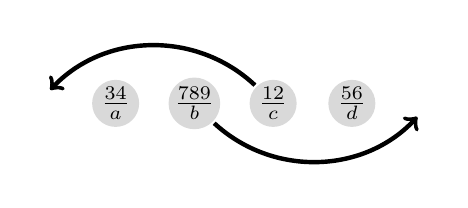
\begin{tikzpicture}[shorten >=1pt,->,ultra thick]
			\tikzstyle{vertex}=[circle,fill=black!15,minimum size=17pt,inner sep=0pt]
			\tikzstyle{vv}=[]
			\foreach \l/\name/\x in {a/34/1, b/789/2, c/12/3, d/56/4}
				\node[vertex] (\name) at (\x,0) {$\frac{\name}{\l}$};
			\node[vv] (s) at (0,0) {};
			\node[vv] (e) at (5,0) {};
			
			\path[every node/.style={font=\sffamily\small}]
			(789) edge[bend right=45] node [right] {} (e)
			(12) edge[bend right=45] node [left] {} (s);
		\end{tikzpicture}


\end{document}

